\begin{enumerate}
\item In $\triangle ABC$ \figref{fig:Fig_2}, $AD \perp BC$. Prove that\\
$AC^2 = AB^2 + BC^2 - 2BC \times BD $
\begin{figure}[H]
    \centering
    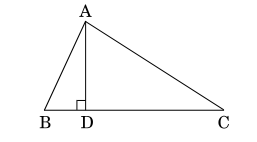
\includegraphics[width=\columnwidth]{figs/cons2.png}
    \caption{}
    \label{fig:Fig_2}
\end{figure}

\item Draw a circle of radius $4$ cm. From a point $6$ cm away from its centre, construct a pair of tangents to the circle and measure their lengths.

\item Construct a triangle with sides $5cm$, $6cm$ and $7cm$ and then another triangle whose sides are $\frac{3}{5}$ of the corresponding sides of the first triangle.

\item Let $\triangle ABC  \thicksim  \triangle DEF$  and their areas be respectively, $64cm^2$ and $121cm^2$. If $EF=15.4cm$, find $BC$.

\item Prove that the sum of the squares of the sides of a rhombus is equal to the sum of the squares of its diagonals. 

\item In \figref{fig:Fig_3}, $BL$ and $CM$ are medians of a $\triangle ABC$ right-angled at $A$. Prove that $4(BL^2 + CM^2)= 5 BC^2$. 
\begin{figure}[H]
    \centering
    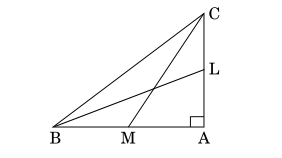
\includegraphics[width=\columnwidth]{figs/cons1.png}
    \caption{Triangle ABC}
    \label{fig:Fig_3}
\end{figure}

\item In  \figref{fig:Figh_1}, $ABC$ is an isosceles triangle right angled at $C$ with $AC = 4 cm$. Find the length of $AB$.
\begin{figure}[H]
    \centering
    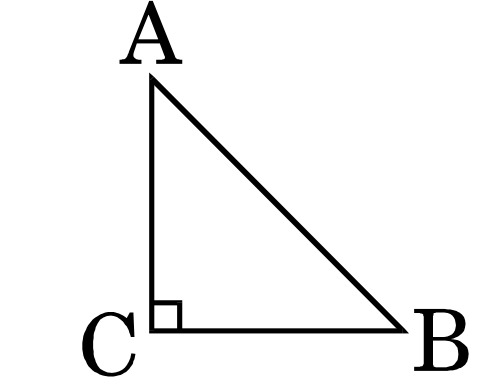
\includegraphics[width=\columnwidth]{figs/img1.jpg}
    \caption{Triangle $ABC$}
    \label{fig:Figh_1}
\end{figure}

\item In  \figref{fig:Figh_2}, $DE \parallel BC$. Find the length of side $AD$, given that $AE = 1.8 cm$, $ BD = 7.2 cm$ and $ CE = 5.4 cm$.
\begin{figure}[H]
    \centering
    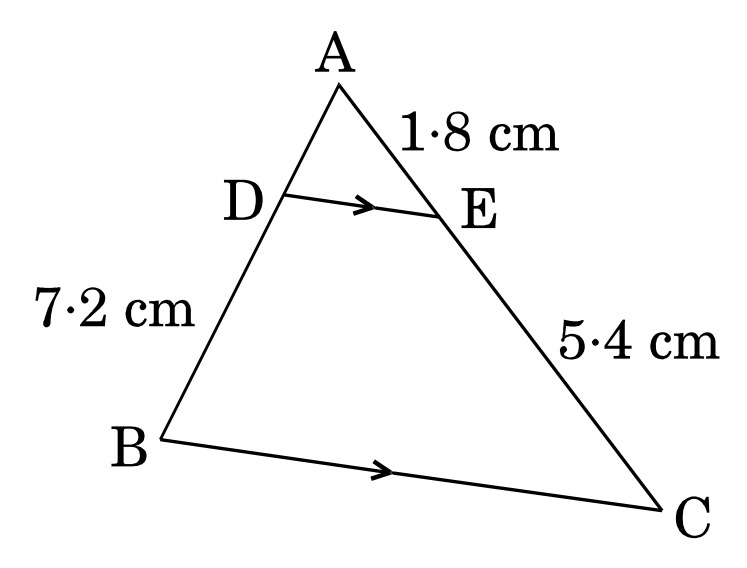
\includegraphics[width=\columnwidth]{figs/img2.jpg}
    \caption{Triangle $ABC$ }
    \label{fig:Figh_2}
\end{figure}

\item Two right triangles $ABC$ and $DBC$ are drawn on the same hypotenuse $BC$ and on the same side of $BC$. If $AC$ and $BD$ intersect at $P$, prove that $AP \times PC = BP \times DP$.

\item Construct an equilateral $\triangle ABC$ with each side $5 cm$. Then construct another triangle whose sides are $\frac{2}{3}$ times the corresponding sides of $\triangle ABC$.

\item Diagonals of a trapezium $PQRS$ intersect each other at the point $O$,
$PQ \parallel RS$ and $PQ = 3RS$. Find the ratio of the areas of triangles $POQ$ and $ROS$.

\item In \figref{fig:Fig-1}, $PS = 3 cm$, $QS = 4 cm$, $\angle$ $PRQ$ = $\theta$, $\angle$ $PSQ$ = $90\degree$, $PQ$ $\perp$ $RQ$ and $RQ = 9 cm$. Evaluate $\tan$ $\theta$.
\begin{figure}[H]
    \centering
    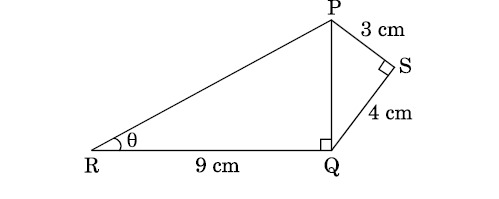
\includegraphics[width=\columnwidth]{figs/Screenshot2023-12-27094821.png}
     \caption{Triangle PSQR}
    \label{fig:Fig-1}
\end{figure}

\item Two concentric circles of radii $a$ and $b$ $\brak{a > b}$ are given. Find the length of the chord of the larger circle which touches the smaller circle.

\item Construct a triangle, the lengths of whose sides are $5 cm$, $6 cm$ and $7 cm$. Now construct another triangle whose sides are $\frac{5}{7}$ times the corresponding sides of the first triangle.

\item If a line is drawn parallel to one side of a triangle to intersect the other two sides in distinct points, prove that the other two sides are divided in the same ratio.

\item Construct a triangle $ABC$ with side $BC = 6 cm$, $AB = 5 cm$ and $\angle ABC = 60\degree$. Then construct another triangle whose sides are $\frac{3}{4}$ of the corresponding sides of the triangle $ABC$

\item The perpendicular from $A$ on side $BC$ of a $\triangle ABC$ meets $BC$ at $D$ such that
$DB = 3CD$. Prove that $2AB^2 = 2AC^2 + BC^2$.

\item $AD$ and $PM$ are medians of triangles $ABC$ and $PQR$ respectively where
$\triangle ABC \sim \triangle PQR$. Prove that ${\frac {AB}{PQ}} = {\frac {AD}{PM}}$.

\item Prove that tangents drawn at the ends of a diameter of a circle are parallel.

\item The area of two similar triangles are $25 sq. cm$ and $121 sq. cm$. Find the
ratio of their corresponding sides.

\item In \figref{fig:Figppr-1}, $E$ is a point on $CB$ produced of an isosceles ${\triangle ABC}$, with side $AB$ = $AC$. If ${AD \perp  BC }$ and ${ EF \perp AC}$, prove that ${\triangle ABD{ \sim }\triangle ECF}$.
 \begin{figure}[H]
    \centering
    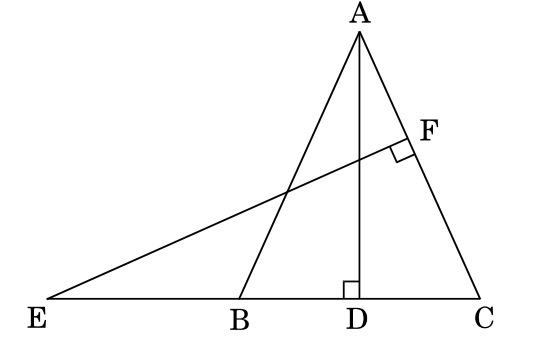
\includegraphics[width=\columnwidth]{figs/Figure_1.png}
    \caption{Triangle}
    \label{fig:Figppr-1}
\end{figure}

\item Prove that the parallelogram circumscribing a circle is a rhombus.

\item In a triangle, if the square of one side is equal to the sum of the squares of the other two sides, then prove that the angle opposite to the first side is a right angle.

\item In two concentric circles, prove that all chords of the outer circle which touch the inner circle, are of equal length.

\item Construct an isosceles triangle whose base is $8 cm$ and altitude $4 cm$ and then another triangle whose sides are $\frac{3}{4}$ times the corresponding sides of the isosceles triangle.

\item Construct a right triangle in which sides (other than the hypotenuse) are $8 cm$ and $6 cm$. Then construct another triangle whose sides are $\frac{5}{3}$ times the corresponding sides of the right triangle.

\item Construct a $\triangle ABC$ in which $CA = 6cm$ , $AB = 5cm$ and $BAC= 45\degree$. Then  construct a triangle whose sides are $\frac{3}{5}$ of the corresponding sides of $\triangle ABC$.
\item Prove that in a right angle triangle, the square of the hypotenuse is equal the sum of squares of the other two sides.
\item In \figref{fig:tri35}, $DE \parallel BC$, $ AD = 1 cm , BD = 2 cm$. What is the ratio of the area of $\triangle ABC$ to the area of $\triangle ADE$?
	\begin{figure}[H]
				\centering
				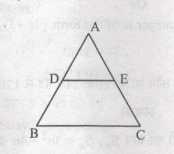
\includegraphics[width=\columnwidth]{figs/tri123.jpeg}
				\caption{triangle}
				\label{fig:tri35}
				
				
			\end{figure} 
\item In \figref{fig:construcion45}, angle $ACB = 90\degree$ and $CD \perp AB$, prove that $CD ^ 2 = BD \times AD$.
	\begin{figure}[H]                                                            \centering
		                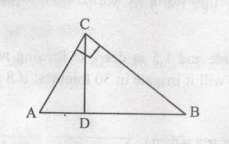
\includegraphics[width=\columnwidth]{figs/i3.jpeg}
				\caption{circles}
				\label{fig:construcion45}
		        \end{figure}
		        
\item Construct a triangle $ABC$ with side $BC = 6 cm$, $\angle B=45\degree, \angle A= 105\degree$. Then construct another triangle whose sides are $\frac{3}{4}$ times the corresponding sides of the $\triangle ABC$
\item Prove that the ratio of the areas of two similar triangles is equal to the square of the ratio of their corresponding sides. 
\end{enumerate}
